\section{Terminology: Risk \& Opportunity Management Process}
\label{sec:process}

This section defines terminology used in describing the management of risks and opportunities at Rubin.
Risks and opportunities are set to have one of the following Risk Register statuses and follow the lifecycle described in Figure \ref{fig:risk-lifecycle}.

\begin{itemize}
	\item \textbf{Candidate} ---
	Risks and opportunities in a draft state, which are not actively managed by the project.

	\item \textbf{Active} ---
	Risks and opportunities deemed valid, and actively managed by the project.

	\item \textbf{Realized} ---
	Risks and opportunities which have been realized.
	There are three models available for the trigger:
		\begin{itemize}
			\item \textbf{Specific Trigger Date} ---
			A specific calendar date when contingency funds must either be obligated to respond to a risk, the risk can be retired, or an opportunity's beneficial event will occur.

			\item \textbf{Random Occurrence} ---
			Certain risks or opportunities are known to potentially occur but their date(s) are random; for example, critical staff may depart the project, weather delay, equipment failure.
			This type of event requires an estimate of the number of random occurrences and the cost of each.

			\item \textbf{Distributed Occurrence} ---
			Identical risks or opportunities are sometimes distributed throughout periods in the project; for example, software packages are evaluated for performance on an annual basis.
			This type of event distributes the possible contingency obligation profile over the specified time span.
		\end{itemize}

	\item \textbf{Retired} ---
	Risks and opportunities which can no longer valid or actively managed, as they have been realized or the event trigger can no longer occur.

	\item \textbf{Deprecated} ---
	Risks and opportunities that were deemed invalid and are were not actively managed.
\end{itemize}

\subsection{Diagram: Risk \& Opportunity Management Process}

\begin{figure}[H]
\caption{Lifecycle of Risks.}
\centering
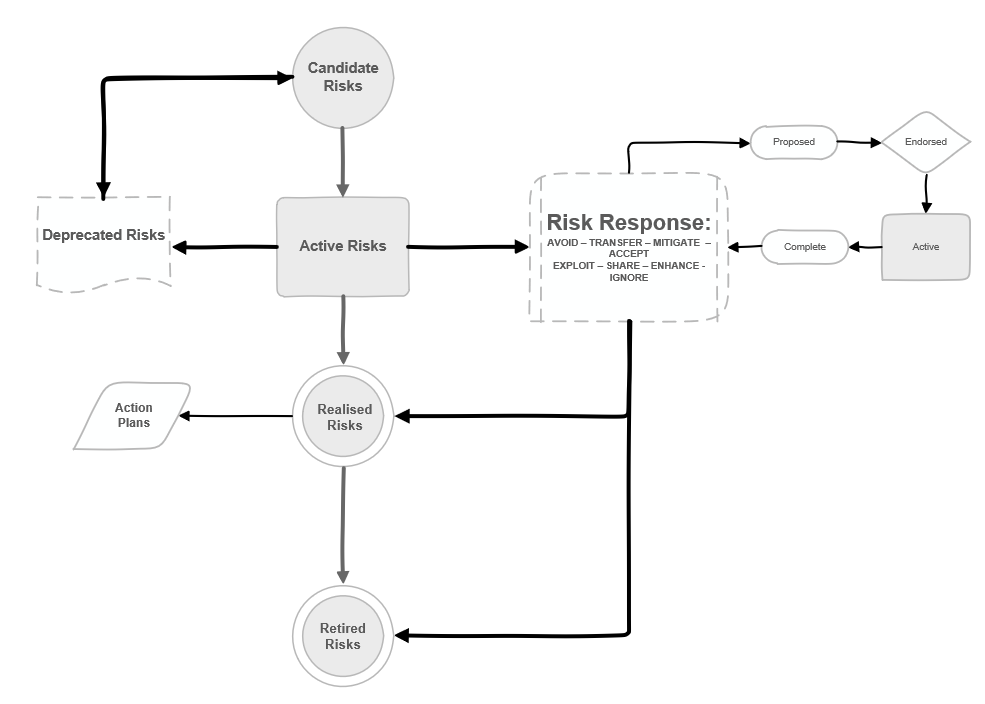
\includegraphics[width=\textwidth]{risk-lifecycle}
\label{fig:risk-lifecycle}
\end{figure}

\subsection{Terminology: Risk Categories}
\label{sec:risk-categories}

The following are categories and subcategories used to define risks in the Risk Register.

\begin{itemize}
	\item \textbf{Program Science} Category
		\begin{itemize}
			\item Astronomy and Astrophysics Community --- Priorities, needs and expectations of the community and the changes related to it.
			\item Science Related --- Science produced by the organization and its relevance and impact.
		\end{itemize}
	\item \textbf{Technical} Category
		\begin{itemize}
			\item Scope --- Related to Scope changes of the Organization/Project objectives.
			\item Requirements --- Identifying/missing/not well defined requirements.
			\item Processes --- Inadequate or not well defined technical or operational processes.
			\item Technology --- Technology readiness level and related.
			\item Interfaces --- Technical interfaces, infrastructure and complexity of the interfaces, and related.
			\item Quality --- Verification of the requirements and concept of operations, to ensure the performance. How well the as-built system compares against the requirements.
		\end{itemize}
	\item \textbf{Management} Category
		\begin{itemize}
			\item Program/Project Management --- Anything related to project and program like schedule, planning, monitoring and controlling.
			\item NOIRLab/AURA Management --- AURA, NOIRLab rates and other AURA and NOIRLab management related.
			\item Operations Management --- Portfolio Management, finance, ITOps, safety group, and other operations related.
			\item Resourcing --- Labor resourcing, shared resources availability, conflicts between fraction of shared resources.
			\item Communication --- Internal communication within the organization and external communication.
			\item Health \& Safety Environment --- Mental health of the employees due to pandemic, safety in the observatories, etc.
		\end{itemize}
	\item \textbf{Commercial/Organizational} Category
		\begin{itemize}
			\item Contractual/Procurement --- All contractual and procurement related events, liabilities, warranties, legal, compliance.
			\item Partnerships and Joint Ventures --- Any risks associated with tenants, partners and in-kind support, relationship.
			\item Subcontracts and Suppliers --- Any risk related to subcontractor and supplier issues (non-contractual); e.g., supplier going bankrupt.
		\end{itemize}
	\item \textbf{External} Category
		\begin{itemize}
			\item Financial --- All sources of risks related to funding and cash flow.
			\item Legislation and Regulatory --- Lease renewals, political, sites \& facilities, applicable law.
			\item Exchange Rates --- Exchange rates for currency, e.g., USD-CLP, USD-EUR.
			\item Natural Environmental Factors --- Risks related to weather, earthquakes, tsunami and other natural factors.
			\item Human Environmental Factors --- Risks related to light pollution, satellites, air pollution and other passive human factors.
			\item External Stakeholders --- External stakeholders influencing like funding agencies, public, protest group, hackers, hostile competitors or other active human factors.
		\end{itemize}
\end{itemize}

\subsection{Terminology: Risk Likelihood and Impact Categories}
\label{sec:risk-impact-tables}

This subsection includes the following tables to define risk likelihood categories and risk impact categories:
\begin{itemize}
	\item Table \ref{table:risk-likelihood} includes the definition of risk likelihood categories and corresponding percent chance.
	\item Table \ref{table:risk-overall-impacts} includes the definition of impact categories based on overall risk.
	\item Table \ref{table:risk-cost-impacts} includes the definition of impact categories based on cost.
	\item Table \ref{table:risk-schedule-impacts} includes the definition of impact categories based on schedule.
	\item Table \ref{table:risk-performance-impacts} includes the definition of impact categories based on performance.
\end{itemize}

\begin{table}[H]
\caption{Risk Likelihood Categories.}
\label{table:risk-likelihood}
\begin{tabular}{lll}
\multicolumn{1}{c}{\textbf{Likelihood Category}} & \multicolumn{1}{c}{\textbf{Percent Chance}} & \multicolumn{1}{c}{\textbf{Definition}} \\
Remote      & 10-20\% & Extremely unlikely to occur.                 \\
Unlikely    & 21-40\% & May occur only in exceptional circumstances. \\
Possible    & 41-60\% & Could occur in certain circumstances.        \\
Likely      & 61-80\% & Probably will occur in many circumstances.   \\
Very Likely & 81-90\% & Expected to occur in most circumstances.    
\end{tabular}
\end{table}

\begin{table}[H]
\caption{Risk Overall Impact Categories.}
\label{table:risk-overall-impacts}
\begin{tabular}{|c|l|}
\hline
\textbf{Impact Category} & \multicolumn{1}{c|}{\textbf{Overall Impact}}                                                                                                    \\ \hline
\textbf{Low}             & \begin{tabular}[c]{@{}l@{}}Any other impacts with respect to operations, project, or\\ initiative within the Programs or Services.\end{tabular} \\ \hline
\textbf{Moderate}        & \begin{tabular}[c]{@{}l@{}}Any impacts with respect to delivering an NOIRLab Program\\ or Service POP milestone.\end{tabular}                   \\ \hline
\textbf{Significant}     & \begin{tabular}[c]{@{}l@{}}Any impacts with respect to Key Performance Evaluation metric(s)\\ of an NOIRLab Program or Service.\end{tabular}    \\ \hline
\textbf{Damaging/Major}  & \begin{tabular}[c]{@{}l@{}}Any impacts with respect to priorities in the POP or LRP of\\ an NOIRLab Program or Service.\end{tabular}            \\ \hline
\textbf{Catastrophic/Extreme} &
  \begin{tabular}[c]{@{}l@{}}Any impacts with respect to NOIRLab Center CA and\\ Programs CSAs, and/or impacting the mission of NOIRLab or\\ any constituent Programs or Services.\end{tabular} \\ \hline
\end{tabular}
\end{table}

\begin{table}[H]
\caption{Risk Cost Impact Categories.}
\label{table:risk-cost-impacts}
\begin{tabular}{|c|l|}
\hline
\textbf{Impact Category}      & \multicolumn{1}{c|}{\textbf{Cost Impact}}                              \\ \hline
\textbf{Low}                  & Minimal consequence.                                                   \\ \hline
\textbf{Moderate}             & Cost variance less than or equal to 5\% of total approved FY baseline. \\ \hline
\textbf{Significant}    & \begin{tabular}[c]{@{}l@{}}Cost variance greater than 5\% but less than or equal to 10\% of total \\ approved FY baseline.\end{tabular} \\ \hline
\textbf{Damaging/Major} & \begin{tabular}[c]{@{}l@{}}Cost variance greater than 10\% but less than or equal to 15\% of total\\ approved FY baseline.\end{tabular} \\ \hline
\textbf{Catastrophic/Extreme} & Cost variance greater than 15\% of total approved FY baseline.         \\ \hline
\end{tabular}
\end{table}

\begin{table}[H]
\caption{Risk Schedule Impact Categories.}
\label{table:risk-schedule-impacts}
\begin{tabular}{|c|l|}
\hline
\textbf{Impact Category} & \multicolumn{1}{c|}{\textbf{Schedule Impact}} \\ \hline
\textbf{Low}             & Minimal consequence.                          \\ \hline
\textbf{Moderate} &
  \begin{tabular}[c]{@{}l@{}}Critical path does not slip; total slack of slipped tasks will not\\ impact critical path in less than 10 days.\end{tabular} \\ \hline
\textbf{Significant} &
  \begin{tabular}[c]{@{}l@{}}Critical path does not slip; total slack of slipped tasks is within\\ 10 days of impacting the critical path.\end{tabular} \\ \hline
\textbf{Damaging/Major}  & Critical path slips.                          \\ \hline
\textbf{Catastrophic/Extreme} &
  \begin{tabular}[c]{@{}l@{}}Critical path slips and one or more critical milestones or events\\ cannot be met.\end{tabular} \\ \hline
\end{tabular}
\end{table}

\begin{table}[H]
\caption{Risk Performance Impact Categories.}
\label{table:risk-performance-impacts}
\begin{tabular}{|c|l|}
\hline
\textbf{Impact Category} &
  \multicolumn{1}{c|}{\textbf{Performance Impact}} \\ \hline
\textbf{Low} &
  Minimal consequence to objectives/goals. \\ \hline
\textbf{Moderate} &
  Minor consequence to objectives/goals. \\ \hline
\textbf{Significant} &
  \begin{tabular}[c]{@{}l@{}}Unable to achieve a particular objective/goal, but remaining objective\\ goals represent better than minimum success or outcome.\end{tabular} \\ \hline
\textbf{Damaging/Major} &
  \begin{tabular}[c]{@{}l@{}}Unable to achieve multiple objectives/goals, but minimum success can\\ still be achieved or claimed.\end{tabular} \\ \hline
\textbf{Catastrophic/Extreme} &
  \begin{tabular}[c]{@{}l@{}}Unable to achieve objectives/goals such that minimum success cannot\\ be achieved or claimed.\end{tabular} \\ \hline
\end{tabular}
\end{table}
